Laravel é um \textit{framework} livre, de código aberto, voltado para desenvolvimento de sistemas baseado em internet e feito em PHP. Tem como principal característica auxiliar no desenvolvimento de aplicações seguras e performáticas de forma rápida, com código limpo e simples, já que ele incentiva o uso de boas práticas de programação e utiliza o padrão PSR-2 como guia para estilo de escrita do código. Foi criado por Taylor Otwell e tem como principal função desenvolver aplicações web com padrão de arquitetura MVC. Algumas características nativas do Laravel são: sua sintaxe descomplicada e concisa, um sistema modular com gerenciador de dependências dedicado, várias formas de acesso a banco de dados relacionais e vários utilitários indispensáveis no auxílio ao desenvolvimento e manutenção de sistemas. O código fonte do Laravel está hospedado no GitHub e licenciado sob os termos da licença MIT \cite{portalgsti:laravel}. 

Segundo \citeonline{locaweb:laravel}, Laravel é o \textit{framework} que está no top \textit{trends} dos mais buscados no Google, isso desde agosto de 2014, que coincide com o ano de lançamento da versão 5.0. Sua divisão em rotas, \textit{controllers} e \textit{models}, sendo compatível com diversos bancos de dados, trabalhando de forma relacional ou orientada a objetos como: MySQL, Postgress, Redis, MongoDB, Cassandra e SQL Server, utilizando \textit{features} Scaffold ou Internacionalização (i18n), faz com que o Laravel seja altamente compatível. Sendo assim, basta ajustar as configurações e definir qual o banco de dados desejado e o sistema mantém seu funcionamento caso a estrutura estiver pronta, utilizando uma implementação simples do ActiveRecord chamada de Eloquent ORM, que é uma ferramenta que traz várias funcionalidades para facilitar a inserção, atualização, busca e exclusão de registros. Para a criação de interface gráfica, o Laravel utiliza uma \textit{engine} de \textit{template} chamada Blade, que traz uma gama de ferramentas que ajudam a criar interfaces bonitas e funcionais de forma rápida e evitar a duplicação de código.

\begin{citacao}
 O Laravel é uma estrutura de aplicativos da web com sintaxe expressiva e elegante. Acreditamos que o desenvolvimento deve ser uma experiência agradável e criativa para ser verdadeiramente gratificante. O Laravel tenta aliviar a dor do desenvolvimento, facilitando tarefas comuns usadas na maioria dos projetos da web \cite{laravel}.
\end{citacao}

Com sua baixa curva de aprendizagem e elegância, seu diferencial é a grande quantidade de recursos nativos que o mesmo contém para auxiliar o processo de desenvolvimento. Além disso, o \textit{framework} tem como objetivo aumentar a velocidade de codificação, sem esquecer características importantes como a segurança e performance da aplicação.

Segundo \citeonline{comparisonLaravel}, afirmaram que ao comparar PHP procedural com CodeIgniter e Laravel, o Laravel tem bom desempenho e menos tempo de execução para todas as quatro ações. Os resultados em milissegundos de dez entradas como média para as quatro ações são apresentados na \autoref{tab:comparisonLaravel}.

\begin{table}[H]
    \centering
    \caption{Resultado do experimento no tempo de execução
    \label{tab:comparisonLaravel}}
    \begin{tabular}{rrrrr}
            \toprule
            & CREATE    & READ      & UPDATE    & DELETE \\
            \midrule
            PLAIN PHP   & 0.066     & 0.063    & 0.0925   & 0.065 \\
            CODEIGNITER & 0.0634    & 0.0747   & 0.0825   & 0.616 \\
            LARAVEL     & 0.201     & 0.222    & 0.312    & 0.301 \\
            \bottomrule
    \end{tabular}
    \fonte{\citeonline{comparisonLaravel}}
\end{table}

\citeonline{He2015/01} também prova a eficácia do método de projeto web com base na estrutura do Laravel, criando um ambiente operacional virtual e comparando com o mesmo ambiente desenvolvido em CodeIgniter. De acordo com a \autoref{fig:He2015/01}, a eficiência do desenvolvimento baseado em Laravel é maior em comparação com o método tradicional de design da web baseado na estrutura do CodeIgniter, justificado pela escalabilidade robusta, de modo a melhorar a eficiência do desenvolvimento.

\begin{figure}[H]
    \centering
    \caption{Tendências de eficiência de desenvolvimento - Laravel e CodeIgniter}
    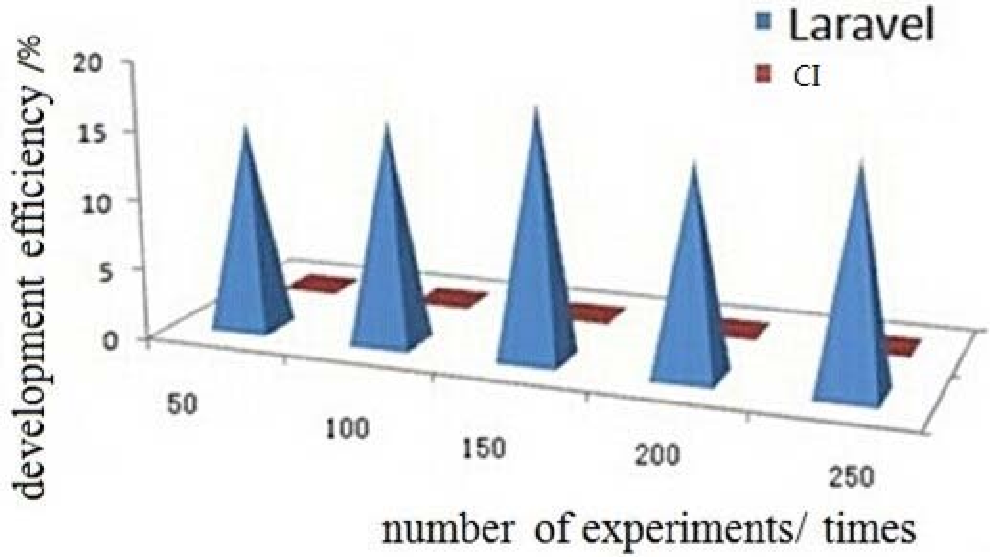
\includegraphics[width=0.6\textwidth]{./dados/figuras/fig9}
    \fonte{\citeonline{He2015/01}}
    \label{fig:He2015/01}
\end{figure}

%%%Para utilização do Laravel é preciso das ferramentas básicas para desenvolvimento em PHP, sugere-se: o XAMPP, pois já incluem o servidor Apache, banco de dados MySql e o próprio PHP, além disso será necessário realizar a instalação do Composer, através do qual é realizada a instalação do Laravel.